\section{Representación en serie de potencias}

Ya se sabe que una serie de potencias tiene un radio de convergencia (llámese $R$). Una función $f$ puede ser representada por una serie de potencias, digamos centrada en $z_0$. Entonces se dice que $f(z)$ está representada por la serie de potencias o que está desarrollada en serie de potencias si 
\begin{equation}
  f(z)=\sum_{n=0}^\infty c_n (z-z_0)^n = c_0 + c_1(z-z_0) + c_2(z-z_0)^2 + \dots
\end{equation}
la función es igual a la suma de la serie de potencias (o bien, la serie converge a $f(z)$). Esta representación es única, es decir, una función no puede representarse por dos series de potencias diferentes con el mismo centro.

\subsection{Series de Taylor}
\label{sec:serie_de_taylor}

A continuación se demostrará que \textbf{toda} función analítica $f(z)$ puede representarse mediante series de potencias, denominadas series de Taylor de $f(z)$ y que son de la misma forma que en \texttt{Cálculo III}, con $x$ sustituida por el complejo $z$.
\begin{theorem}[Serie de Taylor]
  Sea $f(z)$ \textbf{analítica} en un dominio $D$, y sea $z=z_0$ cualquier punto en $D$. Entonces existe exactamente una serie de potencias con centro en $z_0$ que representa a $f(z)$. Esta serie es de la forma 
  $$
  f(z)=\sum_{k=0}^\infty c_k(z-z_0)^k 
  $$
  en donde $c_k=f^{(k)}(z_0)/k!$.

  Esta representación es válida en el mayor disco abierto con centro $z_0$ contenido en $D$. 
\end{theorem}

\begin{proof}
La herramienta importante en la obtención de la fórmula de Taylor es la fórmula de la integral de Cauchy que ya hemos visto:
\begin{equation}
f(z)=\frac{1}{j2\pi} \oint_\Gamma \frac{f(z^\ast)}{z^\ast -z}dz^\ast
\label{eq:formula_integral_cauchy(sec3)}
\end{equation}
Aquí hemos llamado $z^\ast$ a la variable y $z$ al punto (que usualmente llamabamos $z_0$). Un esquema de la situación puede verse en la figura \ref{fig:formula_integral_cauchy(sec3)}.
\begin{figure}[ht]
  \centering
  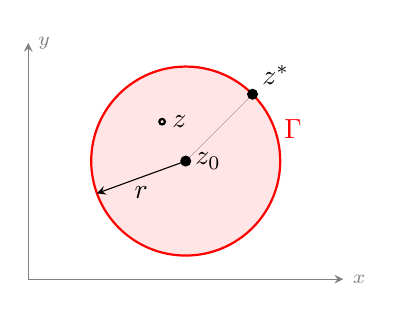
\begin{tikzpicture}[>=stealth]
    \draw[->,gray] (0,0) -- (4,0) node[right] {\scriptsize$x$};
    \draw[->,gray] (0,0) -- (0,3) node[right] {\scriptsize$y$};

    \draw[red,fill=red!10,thick] (2,1.5) circle (1.2);

    \path[red] (2,1.5) -- +(20:1.2) node[right] {$\Gamma$};

    \fill[black] (2,1.5) circle (2pt) node[right] {$z_0$};

    \draw[thick] (1.7,2) circle (1pt) node[right] {$z$};

    \fill[black] (2,1.5) -- +(45:1.2) circle (2pt) node[above right] {$z^\ast$};

    \draw[->] (2,1.5) -- node[below] {$r$} +(200:1.2cm);
  \end{tikzpicture}
  \caption{Esquema de la ecuación \eqref{eq:formula_integral_cauchy(sec3)}}
  \label{fig:formula_integral_cauchy(sec3)}
\end{figure}

Un detalle que será de utilidad es que si observamos la figura \ref{fig:formula_integral_cauchy(sec3)} vemos que la distancia desde el centro ($z_0$) al punto $z$ es en cualquier caso menor que la distancia desde el centro a $z^\ast$, por tanto:
\begin{equation}
  \left\lvert \frac{z-z_0}{z^\ast -z_0} \right\rvert < 1
  \label{eq:distancias_al_centro}
\end{equation}

La siguiente idea es desarrollar $1/(z^\ast - z)$ de la ecuación \eqref{eq:formula_integral_cauchy(sec3)} como serie geométrica. Aplicando algunos pasos algebraicos, primero se obtiene
\begin{equation*}
  \frac{1}{z^\ast -z}= \frac{1}{z^\ast-z_0-(z-z_0)}=\frac{1}{(z^\ast- z_0)\left(1-\frac{z-z_0}{z^\ast -z_0}\right)}
\end{equation*}
Si llamamos $q=\frac{z-z_0}{z^\ast -z_0}$ para mantener una notación más compacta a esta última expresión, podemos escribirla como
\begin{equation}
  \frac{1}{z^\ast -z} = \left(\frac{1}{z^\ast -z_0}\right)\left(\frac{1}{1-q}\right)
  \label{eq:suma_geometrica}
\end{equation}
donde $q$ es la razón de la serie geométrica. Anteriormente, en la ecuación \eqref{eq:distancias_al_centro} hemos dicho que la razón del valor absoluto de las distancias es menor que uno y esto no es más que la razón de la serie geométrica, por lo tanto, la serie geométrica \eqref{eq:suma_geometrica} es convergente. Entonces, podemos escribir la expresión \eqref{eq:suma_geometrica} de la siguiente manera
\begin{equation}
  \frac{1}{z^\ast-z}=\frac{1}{z^\ast -z_0}\sum_{k=0}^\infty \left(\frac{z-z_0}{z^\ast -z_0}\right)^k = \frac{1}{z^\ast -z_0}(1 + q + q^2 \dots )
  \label{eq:serie_geometrica_taylor}
\end{equation}

Ahora que tenemos esta última expresión, podemos escribir $1/(z^\ast-z)$ de la integral de la primera ecuación \eqref{eq:formula_integral_cauchy(sec3)} como \eqref{eq:serie_geometrica_taylor}:
$$
f(z)=\frac{1}{j2\pi} \oint_\Gamma \frac{f(z^\ast)}{z^\ast -z}dz^\ast = \frac{1}{j2\pi} \oint_\Gamma \left(\frac{1}{z^\ast -z_0}\sum_{k=0}^\infty \left(\frac{z-z_0}{z^\ast -z_0}\right)^k\right)\, f(z^\ast)dz^\ast
$$
Y como la serie geométrica es un caso particular de una serie de potencias, también se cumple que cuando es convergente, converge uniformemente. De este modo podemos aplicar las propiedades distributivas y de diferenciación e integración a la sumatoria. Como el factor $1/(z^\ast-z_0)$ está multiplicando la sumatoria, podemos multiplicar cada término de la sumatoria sin modificar su valor. Lo mismo con la integral, integramos término a término en la sumatoria. Con esto, resulta
$$
f(z)=\frac{1}{j2\pi}\sum_{k=0}^\infty \oint_\Gamma \frac{f(z^\ast)(z-z_0)^k}{(z^\ast -z_0)^{k+1}}dz^\ast
$$
Como $(z-z_0)^k$ no depende de $z^\ast$ que es la variable de integración, podemos sacarla de la integral 
$$
f(z)=\sum_{k=0}^\infty \frac{(z-z_0)^k}{j2\pi}\oint_\Gamma \frac{f(z^\ast)}{(z^\ast - z_0)^{k+1}}dz^\ast
$$
Al comparar esta expresión con la ecuación de la derivada $n$-ésima de Cauchy
$$
f^{(n)}(z_0)=\frac{n!}{j2\pi}\oint_\Gamma \frac{f(z)}{(z-z_0)^{n+1}}dz
$$
vemos que podemos realizar la siguiente sustitución:
$$
f(z)=\sum_{k=0}^\infty \frac{(z-z_0)^k}{k!}\left[\frac{k!}{j2\pi}\oint_\Gamma \frac{f(z^\ast)}{(z^\ast - z_0)^{k+1}}dz^\ast\right] = \sum_{k=0}^\infty (z-z_0)^k\frac{f^{(k)}(z_0)}{k!}
$$
Y así, hemos llegado a la serie de Taylor para funciones de variable compleja. En notación compacta se escribe como
$$
\boxed{\sum_{k=0}^\infty c_k(z-z_0)^k}
$$
donde $c_k=f^{(k)}(z_0)/k!$.
\end{proof}

Se dice que una función compleja es \textit{analítica} en $z_0$ si tiene un desarrollo en serie de potencias en algún disco abierto alrededor de $z_0$. Se acaba de probar que una función que es diferenciable en un disco abierto alrededor de un punto es analítica en ese punto.

Solo se han calculado los coeficientes de una serie de Taylor por las fórmulas de derivación o integración. Cuando es posible, en la práctica se usan series conocidas y operaciones tales como diferenciación e integración para obtener una representación en serie de una función. Esta estrategia hace uso del siguiente teorema sobre la unicidad de las representaciones en serie de potencias.
\begin{theorem}[Unicidad de la serie de Taylor]
  Suponemos que, en algún disco $\lvert z-z_0\rvert < r$, $f$ tiene dos representaciones en serie de Taylor
  $$
  \sum_{k=0}^\infty c_n(z-z_0)^k \qquad \sum_{k=0}^\infty d_n (z-z_0)^k
  $$
  Entonces para $k=0,1,2,\dots$ tenemos que 
  $$
  c_k = \frac{f^{(k)}(z_0)}{k!} \qquad d_k = \frac{f^{(k)}(z_0)}{k!}
  $$
  Entonces las dos series son iguales (ya que sus coeficientes son iguales). Por tanto una función $f$ que puede ser representada en serie de Taylor centrada en un punto $z_0$ tiene una única representación.
\end{theorem}

Ahora veamos algunos ejemplos. 

\begin{example}
  Encontrar el desarrollo de Taylor de $f(z)=e^z$ alrededor de $z=j$.

  Se sabe que para todo $z$, 
  $$
  e^z = \sum_{n=0}^\infty \frac{z^n}{n!}
  $$
  Para un desarrollo alrededor de $j$, la serie de potencias debe estar en términos de potencias de $z-j$. De esta manera 
  $$
  e^z = e^{z-j+j}=e^j e^{z-j}=\sum_{n=0}^\infty \frac{e^j}{n!}(z-j)^n
  $$
  Esta serie converge para todo $z$.

  En este ejemplo, hubiera sido igual de fácil calcular los coeficientes de Taylor directamente:
  $$
  c_n = \frac{f^{(n)}(j)}{n!} = \frac{e^j}{n!}
  $$
  \label{ej:desplazamiento_serie_de_taylor}
\end{example}

\begin{example}
  Escribir la serie de Maclaurin para $f(z)=\cos(z^3)$.

  Un desarrollo de Maclauin es una serie de Taylor alrededor de cero. Para todo $z$,
  $$
  \cos(z)=\sum_{n=0}^\infty \frac{(-1)^n}{(2n)!}z^{2n}
  $$
  Todo lo que se necesita hacer es reemplazar $z$ con $z^3$:
  $$
  \cos(z^3)=\sum_{n=0}^\infty \frac{(-1)^n}{(2n)!}z^{6n}
  $$
  Como es un desarrollo alrededor del origen, es el desarrollo que se buscaba.
  \label{ej:sustitucion_serie_de_taylor}
\end{example}

Si ha prestado atención, en estos ejemplos no hemos necesitado desarrollar o encontrar la ley de formación de los términos $c_n$, hemos usado el conocimiento que tenemos para desarrollar series de Taylor en variable real, y la hemos reemplazado por la variable compleja. En la mayor parte de los casos puede ser complicado o consumir mucho tiempo determinar los coeficientes de la serie de Taylor a partir de la fórmula en el teorema de Taylor, y existen formas mejores y más rápidas para efectuar lo anterior. A continuación se mostraran algunos ejemplos útiles para aplicar distintos métodos y obtener el desarrollo en serie de Taylor.

\subsection{Métodos prácticos para representar en serie de Taylor}

El primer ejemplo \ref{ej:desplazamiento_serie_de_taylor} usa un sencillo método denominado método del \textit{desplazamiento}. Corremos el centro de una serie conocida a otro centro pedido.

El ejemplo \ref{ej:sustitucion_serie_de_taylor} es un claro ejemplo del segundo método, denominado el método de \textit{sustitución}, que consiste en tener el desarrollo de una función determinada $f(z)$ con la cual es posible desarrollar otra función $g(z)$ tal que, como en el caso del ejemplo $f(z^n)=g(z)$ y reemplazar o sustituir la variable.

\begin{example}(Método de desarrollo en serie geométrica)
  Desarrollar 
  $$
  f(z)=\frac{1}{c-bz}
  $$ 
  en potencias de $(z-a)$, en donde $c-ab\neq 0$ y $b\neq 0$.

  Para obtener potencias de $z-a$, se aplica álgebra simple:
  $$
  \frac{1}{c-bz}=\frac{1}{c-ab-b(z-a)}=\frac{1}{(c-ab)\left(1-\frac{b(z-a)}{c-ab}\right)}
  $$
  A la última expresión, si llamamos $q=\frac{b(z-a)}{c-ab}$, entonces $q$ es la razón de una serie geométrica, y se la puede desarrollar tal que
  $$
  \frac{1}{1-q}=\sum_{n=0}^\infty q^n = \sum_{n=0}^\infty \left(\frac{b(z-a)}{c-ab}\right)^n
  $$
  Así, resulta 
  $$
  \frac{1}{c-bz}=\frac{1}{(c-ab)\left(1-\frac{b(z-a)}{c-ab}\right)} = \frac{1}{(c-ab)}\sum_{n=0}^\infty \left(\frac{b(z-a)}{c-ab}\right)^n
  $$
  Y por último, podemos introducir el factor dentro de la serie, siendo entonces 
  $$
  \frac{1}{c-bz}=\sum_{n=0}^\infty \frac{(b(z-a))^n}{(c-ab)^{n+1}}
  $$
  Quedando así desarrollada la expresión.
\end{example}

\begin{example}(Método de integración)
  Encontrar la serie de Maclaurin de $f(z)=\tan^{-1}(z)$. 

  El primer coeficiente es $c_1=f'(z)$, y la derivada de $f$ es 
  $$
  \frac{1}{1+z^2}
  $$
  Si se integra este último resultado, evidentemente se vuelve a obtener $f$, entonces podemos desarrollar la serie de Taylor de este último resultado (desarrollaremos como serie geométrica en este caso) y luego integrar término a término. 
  $$
  \frac{1}{1+z^2}=\frac{1}{1-(-z^2)}=\sum_{n=0}^\infty (-z^2)^n = \sum_{n=0}^\infty (-1)^n z^{2n}
  $$
  Ahora, integrando término a término (usando la integral indefinida para obtener la primitiva), tenemos 
  \begin{align*}
    \int\frac{1}{1+z^2}dz&=\int\sum_{n=0}^\infty (-1)^n z^{2n}dz \\ 
    \tan^{-1}(z) &= \sum_{n=0}^\infty \frac{(-1)^n}{(2n+1)}z^{2n+1}
  \end{align*}
  Esta serie representa el valor principal de $w=u+jv=\tan^{-1}(z)$, definido como el valor para el que $\lvert u \rvert < \pi/2$.
\end{example}
